\documentclass[11pt,letterpaper]{article}
\usepackage[lmargin=1in,rmargin=1in,tmargin=1in,bmargin=1in]{geometry}
\usepackage{../style/homework}
\usepackage{../style/commands}
\setbool{quotetype}{false} % True: Side; False: Under
\setbool{hideans}{false} % Student: True; Instructor: False

% -------------------
% Content
% -------------------
\begin{document}

\homework{13: Due 11/10}{\dots there is no apparent reason why one number is prime and another not. To the contrary, upon looking at these numbers one has the feeling of being in the presence of one of the inexplicable secrets of creation.}{Don Zagier}

% Problem 1
\problem{10} Showing all your work and fully justifying your reasoning, complete the following:
	\begin{enumerate}[(a)]
	\item Using the definition of even, show that $-484$ is even.
	\item Using the definition of odd, show that 151 is odd.
	\item Find the prime factorization of 360. 
	\item Find all the prime divisors of 45!. 
	\item Can an integer of the form $n^4 - 9$, where $n \in \mathbb{Z}$, be prime?
	\end{enumerate} \pspace

\sol 
\begin{enumerate}[(a)]
\item 
\item 
\item 
\item 
\item 
\end{enumerate}



\newpage



% Problem 2
\problem{10} Showing all your work and fully justifying your reasoning, complete the following:
	\begin{enumerate}[(a)]
	\item List at least ten multiples of 17.
	\item List the divisors of 120.
	\item What are the prime divisors of 120?
	\end{enumerate} \pspace

\sol 
\begin{enumerate}[(a)]
\item The multiples of 17 are the integers of the form $17k$, where $k \in \mathbb{Z}$. Choosing $k= -5, -4, \ldots, 5$, we obtain\dots
	\[
	-85, \; -68, \; -51, \; -34, \; -17, \; 0, \; 17, \; 34, \; 51, \; 68, \; 55
	\] \pspace

\item The divisors of 120 are the integers $a$ such that $a \mid 120$. But then the divisors of 120 are 1, 2, 3, 4, 5, 6, 8, 10, 12, 15, 20, 24, 30, 40, 60, and 120. Alternatively, finding the prime factorization of 120, we obtain $120= 2^3 \cdot 3^1 \cdot 5^1$. Then the divisors of 120 are the integers of the form $2^a \cdot 3^b \cdot 5^c$, where $0 \leq a \leq 3$, $0 \leq b \leq 1$, and $0 \leq c \leq 1$. \pspace

\item The prime divisors of 120 are the integers $a$ such that $a \mid 120$ and $a$ is prime. We find the prime factorization of 120: 
	\[
	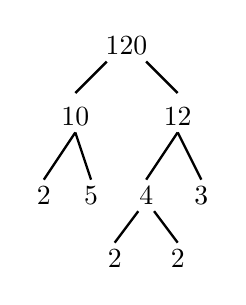
\begin{tikzpicture}
	\node at (-0.15,0.1) {$120$};
	\draw[line width=0.03cm] (-0.4,-0.1) -- (-0.8,-0.5);
	\node at (-0.8,-0.8) {$10$};
	\draw[line width=0.03cm]  (0.1,-0.1) -- (0.5,-0.5);
	\node at (0.5,-0.8) {$12$};
		
	\draw[line width=0.03cm] (-0.8,-1) -- (-1.2,-1.6);
	\node at (-1.2,-1.8) {$2$};
	\draw[line width=0.03cm] (-0.8,-1) -- (-0.6,-1.6);
	\node at (-0.6,-1.8) {$5$};
	
	\draw[line width=0.03cm] (0.5,-1) -- (0.1,-1.6);
	\node at (0.1,-1.8) {$4$};
	\draw[line width=0.03cm] (0.5,-1) -- (0.8,-1.6);
	\node at (0.8,-1.8) {$3$};
	
	\draw[line width=0.03cm] (0,-2.0) -- (-0.3,-2.4);
	\node at (-0.3,-2.6) {$2$};
	\draw[line width=0.03cm] (0.2,-2.0) -- (0.5,-2.4);
	\node at (0.5,-2.6) {$2$};
	\end{tikzpicture}
	\] 
Therefore, $120= 2^3 \cdot 3 \cdot 5$. Then the prime divisors of 120 are 2, 3, and 5. 
\end{enumerate}



\newpage



% Problem 3
\problem{10} Showing all your work and justifying your reasoning, complete the following:
	\begin{enumerate}[(a)]
	\item By enumerating the divisors of 40 and 100, compute $\gcd(40, 100)$.
	\item By enumerating sufficient multiples of 25 and 60, compute $\lcm(25, 60)$.
	\item Compute $\gcd(2^{100} \cdot 3^{200} \cdot 5^{600} \cdot 11^{100},\, 2^{300} \cdot 3^{100} \cdot 5^{600} \cdot 7^{800})$. 
	\item Compute $\lcm(2^{100} \cdot 3^{200} \cdot 5^{600} \cdot 11^{100},\, 2^{300} \cdot 3^{100} \cdot 5^{600} \cdot 7^{800})$. 
	\end{enumerate} \pspace

\sol 
\begin{enumerate}[(a)]
\item Enumerating the divisors of 40 and 100, we have\dots
	\[
	\begin{aligned}
	40&\colon 1, \; 2, \; 4, \; 5, \; 8, \; 10, \; \mathbf{20}, \; 40 \\
	100&\colon 1, \; 2, \; 4, \; 5, \; 10, \; \mathbf{20}, \; 25, \; 50, \; 100
	\end{aligned}
	\]
Therefore, $\gcd(40, 100)= 20$. \pspace

\item Enumerating multiples of 25 and 60, we have\dots
	\[
	\begin{aligned}
	25&\colon 0, \; 25, \; 50, \; 75, \; 100, \; 125, \; 150, \; 175, \; 200, \; 225, \; 250, \; 275, \; \mathbf{300}, \; 325, \; 350, \; 375, \; \ldots \\
	60&\colon 0, \; 60, \; 120, \; 180, \; 240, \; \mathbf{300}, \; 360, \; 420, \; 480, \; 540, \; 600, \; 660, \; 720, \; 780, \; 840, \; 900, \; \ldots
	\end{aligned}
	\]
Therefore, $\lcm(25, 60)= 300$. \pspace

\item Using the fact that if $a= \prod_{i=1}^n p_i^{a_i}$ and $b= \prod_{i=1}^n p_i^{b_i}$, where the $p_i$ are prime and $a_i, b_i \geq 0$, then $\gcd(a, b)= \prod_{i=1}^n p_i^{\min(a_i, b_i)}$, we have\dots
	\[
	\gcd(2^{100} \cdot 3^{200} \cdot 5^{600} \cdot 11^{100},\, 2^{300} \cdot 3^{100} \cdot 5^{600} \cdot 7^{800})= 2^{100} \cdot 3^{100} \cdot 5^{600} \cdot 7^0 \cdot 11^0= 2^{100} \cdot 3^{100} \cdot 5^{600}
	\] \pspace

\item Using the fact that if $a= \prod_{i=1}^n p_i^{a_i}$ and $b= \prod_{i=1}^n p_i^{b_i}$, where the $p_i$ are prime and $a_i, b_i \geq 0$, then $\lcm(a, b)= \prod_{i=1}^n p_i^{\max(a_i, b_i)}$, we have\dots
	\[
	\gcd(2^{100} \cdot 3^{200} \cdot 5^{600} \cdot 11^{100},\, 2^{300} \cdot 3^{100} \cdot 5^{600} \cdot 7^{800})= 2^{300} \cdot 3^{200} \cdot 5^{600} \cdot 7^{800} \cdot 11^{100} 
	\] 
\end{enumerate}



\newpage



% Problem 4
\problem{10} Showing all your work and justifying your reasoning, complete the following:
	\begin{enumerate}[(a)]
	\item Prove or disprove: if $p$ is prime, then $p^2 + 1$ is also prime. 
	\item Using the fact that $ab= \lcm(a, b) \cdot \gcd(a, b)$ and $\gcd(196, 1320)= 4$, compute $\lcm(196, 1320)$. 
	\item If $a, b \in \mathbb{Z}$ such that $\gcd(a, b)= p$, where $p$ is prime, what are the possible values for $\gcd(a^2, b)$, $\gcd(a, b^2)$, $\gcd(a^2, b^2)$, and $\gcd(a^2, b^3)$? 
	\end{enumerate} \pspace

\sol 
\begin{enumerate}[(a)]
\item The statement is false. For instance, $p= 3$ is prime but $3^2 + 1= 10$ is not prime, i.e. composite. \pspace

\item We have\dots
	\[
	\lcm(196, 1320)= \dfrac{196 \cdot 1320}{\gcd(196, 1320)}= \dfrac{258720}{4}= 64680
	\] \pspace

\item If $\gcd(a, b)= p$ is prime, then we know that $p \mid a$ and $p \mid b$. But then we can write $a= Ap^r$ and $b= Bp^s$, where $A, B, r, s \in \mathbb{Z}$, $\gcd(A, p)= 1$, $\gcd(B, p)= 1$, and $r, s \geq 1$. Clearly, we cannot have $r, s \geq 2$ simultaneously; otherwise, we would have $\gcd(a, b)= \gcd(Ap^r, Bp^s) \geq p^2$, a contradiction. Therefore, one of $r$ or $s$ is 1. By possibly relabeling, we suppose that $a= Ap$ and $b= Bp^s$, where $s \geq 1$. \pspace
\end{enumerate}


\end{document}